\documentclass[journal]{IEEEtran}
\usepackage[utf8]{inputenc}
\usepackage[T1]{fontenc}
\usepackage[spanish,es-nodecimaldot,es-noshorthands]{babel}
\usepackage{graphicx}
\usepackage{amsmath}
\usepackage{booktabs}
\usepackage{multirow}
\usepackage{array}
\newcolumntype{L}[1]{>{\raggedright\arraybackslash}p{#1}}
\usepackage{cite}
\usepackage{url}

\renewcommand{\abstractname}{Resumen}
\renewcommand{\IEEEkeywordsname}{Palabras clave}
\renewcommand{\tablename}{Cuadro}
\graphicspath{{figuras/}}

\begin{document}

\title{Estimación del Riesgo de Diabetes Tipo 2 a partir de Factores Demográficos, Antropométricos y de Estilo de Vida Mediante Aprendizaje de Máquina}

\author{Alejandro Gallego Alarcón, Andrés Eduardo Pabón Roldán, Paula Andrea Guarín Guarín
\thanks{Ingeniería de Sistemas, Universidad de Antioquia, Medellín/Caucasia, Colombia.}}

\markboth{}{}

\maketitle

\begin{abstract}
En este trabajo se construye un clasificador que estima si un adulto tiene diabetes a partir de once preguntas del \textit{Behavioral Risk Factor Surveillance System} (BRFSS) 2025 sobre su perfil demográfico, su índice de masa corporal y sus hábitos, con la idea de usarlo como tamizaje inicial sin exámenes de laboratorio. Tras excluir la diabetes gestacional y la prediabetes quedan 342.539 registros, de los cuales el 15,13\% son casos positivos. Se compararon regresión logística, KNN, bosque aleatorio, red neuronal y SVM con kernel RBF, con validación cruzada estratificada, el desbalance corregido dentro de cada pliegue y un conjunto de prueba reservado desde el inicio. Los cinco modelos llegan a un AUC de 0,77 en prueba, sin diferencias significativas entre ellos; la SVM es la que más casos detecta, con una sensibilidad de 0,80. SMOTE no mejoró frente a la ponderación de clases. En la reducción de dimensión, retirar sexo, frutas y vegetales no cambia el desempeño; PCA lo conserva con 45 componentes en la regresión logística y 20 en la SVM, y UMAP pierde entre 7 y 13 puntos de AUC en su versión estándar y sobreajusta en la supervisada. El desempeño parece limitado por la información que traen las variables de encuesta más que por el modelo.
\end{abstract}

\begin{IEEEkeywords}
diabetes tipo 2, aprendizaje supervisado, BRFSS, desbalance de clases, reducción de dimensión.
\end{IEEEkeywords}

\section{Introducción}

\subsection{Contexto y descripción del problema}
La diabetes tipo 2 reúne entre el 90\% y el 95\% de los casos diagnosticados de diabetes y es, a la vez, la forma que más se puede prevenir: buena parte de su riesgo depende del peso, la actividad física y la alimentación, factores que la persona puede modificar \cite{xie2019}. La dificultad está en saber a tiempo quién está en riesgo, porque eso suele exigir exámenes de laboratorio que no todo el mundo tiene a la mano. Un modelo entrenado con datos de encuesta, sin pruebas clínicas, puede servir como un primer filtro de bajo costo que señale a quién conviene remitir a una evaluación más completa; no reemplaza el diagnóstico médico, pero ayuda a priorizar.

Este trabajo usa el \textit{Behavioral Risk Factor Surveillance System} (BRFSS), la encuesta telefónica que los Centros para el Control y la Prevención de Enfermedades (CDC) de Estados Unidos aplican cada año a cientos de miles de adultos. La diabetes tipo 2 aparece ligada de forma consistente a la edad, el índice de masa corporal (IMC), la actividad física, la dieta y el consumo de tabaco o alcohol \cite{majcherek2025}, y todas esas variables están en el BRFSS. El problema concreto es estimar, a partir de once variables demográficas (sexo, edad, raza/etnia, educación, ingreso), antropométricas (categoría de IMC) y de estilo de vida (actividad física, tabaquismo, alcohol, frutas y vegetales) de la edición 2025, si un respondiente tiene diabetes diagnosticada.

\subsection{Paradigma de aprendizaje}
Como la respuesta a la pregunta de diagnóstico está disponible para casi todos los registros, el problema se aborda con aprendizaje supervisado, en la forma de una clasificación binaria (diabetes sí/no). Ignorar esa etiqueta, como haría un enfoque no supervisado, no tendría sentido; tampoco hay escasez de etiquetas que justifique uno semisupervisado, ni un agente que actúe de forma secuencial sobre un entorno, como exigiría el aprendizaje por refuerzo.

El resto del documento está organizado así: la Sección~\ref{sec:datos} describe la base de datos; la \ref{sec:estado}, los trabajos previos y qué se tomó de ellos; la \ref{sec:entrenamiento}, el diseño experimental y los resultados de los cinco modelos; la \ref{sec:reduccion}, la reducción de dimensión, y la \ref{sec:conclusiones}, la discusión y las conclusiones.

\section{Datos}\label{sec:datos}
Se usó el archivo público del BRFSS 2025, que combina las encuestas de línea fija y celular de 47 estados, el Distrito de Columbia, Guam y Puerto Rico. California, Misisipi, Nevada y las Islas Vírgenes no alcanzaron el mínimo de datos requerido ese año y no aparecen, lo que limita un poco la representatividad nacional. El archivo trae 356.158 registros y 284 variables. De ellas se tomaron once predictoras, todas de las variables calculadas por el CDC (prefijo \texttt{\_}), porque ya vienen con categorías agrupadas y un código de faltante consistente (Cuadro~\ref{tab:variables}). Por eso, por ejemplo, el ingreso tiene 7 rangos (\texttt{\_INCOMG1}) y la educación 4 niveles (\texttt{\_EDUCAG}), en lugar de los 11 y 6 de las preguntas originales.

\begin{table}[!t]
\centering
\caption{Variables predictoras, número de categorías válidas y porcentaje de datos faltantes en la muestra analítica (N = 342.539)}
\label{tab:variables}
\footnotesize
\setlength{\tabcolsep}{3pt}
\begin{tabular}{@{}llcr@{}}
\toprule
\textbf{Grupo} & \textbf{Variable (código BRFSS)} & \textbf{Niveles} & \textbf{Falt.} \\
\midrule
Demográfica & Sexo (\texttt{\_SEX}) & 2 & 0,00\% \\
 & Edad, grupos de 5 años (\texttt{\_AGEG5YR}) & 13 & 1,86\% \\
 & Raza/etnia (\texttt{\_RACEGR3}) & 5 & 2,31\% \\
 & Nivel educativo (\texttt{\_EDUCAG}) & 4 & 0,58\% \\
 & Ingreso (\texttt{\_INCOMG1}) & 7 & 19,88\% \\
Antropom. & Categoría de IMC (\texttt{\_BMI5CAT}) & 4 & 9,10\% \\
Estilo de vida & Actividad física (\texttt{\_TOTINDA}) & 2 & 0,26\% \\
 & Fumador (\texttt{\_SMOKER3}) & 4 & 5,80\% \\
 & Alcohol excesivo (\texttt{\_RFDRHV9}) & 2 & 8,10\% \\
 & Frutas $\geq$1 vez/día (\texttt{\_FRTLT1A}) & 2 & 13,05\% \\
 & Vegetales $\geq$1 vez/día (\texttt{\_VEGLT1A}) & 2 & 15,03\% \\
\bottomrule
\end{tabular}
\end{table}

La variable objetivo, \texttt{DIABETE4}, corresponde a la pregunta ``¿Alguna vez un médico le ha dicho que tiene diabetes?''. En toda la encuesta hay 51.827 respuestas ``sí'', 2.671 ``sí, solo durante el embarazo'', 290.712 ``no'', 10.166 ``prediabetes'' y 782 entre ``no sabe'', ``rehusó'' y en blanco. Se dejaron por fuera la diabetes gestacional, porque es transitoria, y la prediabetes, siguiendo a Xie et al. \cite{xie2019}, de modo que la clase positiva solo contiene diagnósticos consolidados. La muestra analítica queda en 342.539 registros: 51.827 positivos (15,13\%) y 290.712 negativos (84,87\%), un desbalance moderado parecido al que reportan Chowdhury et al. \cite{chowdhury2024} en años anteriores.

En el BRFSS, ``no sabe'' y ``rehusó'' tienen un código propio (9 en casi todas las variables y 14 en la edad), y en \texttt{\_BMI5CAT} el faltante es una celda vacía. Todos se unificaron como dato faltante. Ingreso, vegetales y frutas son las variables con más faltantes (13\% a 20\%); el resto está por debajo del 10\%. Cómo se trataron y codificaron se explica en la Sección~\ref{sec:prep}.

\section{Estado del Arte}\label{sec:estado}
Se revisaron cuatro artículos de revista que predicen diabetes con el BRFSS; el Cuadro~\ref{tab:estado} los resume. Xie et al. \cite{xie2019} trabajan casi el mismo problema que este proyecto, diabetes tipo 2 con 138.146 respondientes de 2014: comparan SVM, árbol de decisión, regresión logística, bosque aleatorio, red neuronal y Naive Bayes con una partición \textit{holdout} 2/3--1/3, y aplican SMOTE solo sobre el entrenamiento. Su red neuronal tiene el mejor AUC (0,79) pero la peor sensibilidad, mientras que el árbol, con la menor exactitud, es el que más positivos detecta (51,6\%). Majcherek et al. \cite{majcherek2025} prueban dieciocho algoritmos sobre 253.680 registros de 2015, con partición 80/20 y validación cruzada estratificada; Extra Trees alcanza más de 90\% de exactitud y AUC de 0,99, y el análisis SHAP señala al IMC, la edad, la salud general y el ingreso como las variables de mayor peso. Chowdhury et al. \cite{chowdhury2024} se centran en el desbalance (18\% de positivos en 438.693 registros de 2021): comparan SMOTEN, ENN, SMOTE-Tomek y SMOTE-ENN aplicadas después de partir los datos, documentan que balancear antes de partir infla las métricas, y con ENN y \textit{gradient boosting} suben la sensibilidad de 57,5\% a 71,7\%. Ekambaram et al. \cite{ekambaram2026} comparan árboles, bosque aleatorio, XGBoost y \textit{gradient boosting} con una red convolucional sobre más de 400.000 registros; la red llega a 93,34\% de exactitud, aunque el resumen no detalla la validación ni cómo se trató el desbalance.

\begin{table}[!t]
\centering
\caption{Resumen de los trabajos revisados (Exact.: exactitud; Sens.: sensibilidad)}
\label{tab:estado}
\footnotesize
\setlength{\tabcolsep}{2.5pt}
\begin{tabular}{@{}L{1.5cm}L{1.3cm}L{1.8cm}L{1.85cm}L{1.55cm}@{}}
\toprule
\textbf{Trabajo} & \textbf{Datos} & \textbf{Modelos} & \textbf{Validación y desbalance} & \textbf{Mejor resultado} \\
\midrule
Xie et al. \cite{xie2019} & BRFSS 2014, 138.146 & SVM, árbol, RL, RF, red neuronal, NB & \textit{Holdout} 2/3--1/3; SMOTE en entrenamiento & Exact. 74--82\%; AUC 0,79 \\
\addlinespace
Majcherek et al. \cite{majcherek2025} & BRFSS 2015, 253.680 & 18 modelos (RL, KNN, ensambles) & 80/20 y VC estratificada; SHAP & Extra Trees: exact. $>$90\%, AUC 0,99 \\
\addlinespace
Chowdhury et al. \cite{chowdhury2024} & BRFSS 2021, 438.693 & RL, RF, GB, AdaBoost & 80/20; 4 técnicas de balanceo tras partir & GB + ENN: sens. 71,7\% \\
\addlinespace
Ekambaram et al. \cite{ekambaram2026} & BRFSS, $>$400.000 & Árbol, RF, XGBoost, GB, CNN & No detallada en el resumen & CNN: exact. 93,34\% \\
\bottomrule
\end{tabular}
\end{table}

De esta revisión salen cuatro decisiones concretas para el diseño experimental. Primera, de Chowdhury et al. y Xie et al.: todo balanceo, imputación o codificación se ajusta dentro de un \textit{pipeline}, solo con los datos de entrenamiento de cada pliegue, y el conjunto de prueba se aparta desde el inicio. Segunda, del contraste que muestran Xie et al. entre AUC y sensibilidad: el AUC se usa para elegir hiperparámetros, pero la sensibilidad se vigila como métrica clave. Tercera, como Chowdhury et al. no encuentran que el sobremuestreo sintético sea siempre la mejor opción, se compara SMOTE contra la ponderación de clases antes de adoptarlo. Cuarta, como los resultados de exactitud cercanos a 90\% o más vienen de trabajos que no reportan la sensibilidad ni el manejo del desbalance, la exactitud no se usa como criterio de selección.

\section{Entrenamiento y Evaluación de Modelos}\label{sec:entrenamiento}

\subsection{Configuración experimental}

\subsubsection{Preprocesamiento, codificación e imputación}\label{sec:prep}
Las once predictoras son categóricas y se codificaron de tres maneras, resumidas en el Cuadro~\ref{tab:codif_def}. En la codificación A ninguna variable se imputa: el faltante se convierte en una categoría más, ``no reportado'', y todas pasan a \textit{one-hot}; así, sexo genera 2 columnas, cada binaria de estilo de vida (actividad física, alcohol, frutas y vegetales) 3 (sí, no, no reportado), raza/etnia 6 y fumador 5. En las codificaciones B y C, edad, educación, ingreso e IMC se tratan como enteros estandarizados porque tienen un orden natural, y las nominales siguen en \textit{one-hot}; los faltantes se imputan con la moda global de cada variable. Se usó la moda y no la mediana porque las variables son categóricas, y se descartó imputar con la moda de cada clase porque al predecir la clase es desconocida y usarla en el ajuste filtraría la etiqueta. C agrega además un indicador binario de faltante por variable.

\begin{table}[!t]
\centering
\caption{Codificaciones evaluadas y número de columnas que produce cada una}
\label{tab:codif_def}
\footnotesize
\setlength{\tabcolsep}{2.5pt}
\begin{tabular}{@{}L{2.4cm}L{2.6cm}L{3.5cm}@{}}
\toprule
\textbf{Variables} & \textbf{A: \textit{one-hot} + no reportado} & \textbf{B / C: ordinal + moda (C: + indicador)} \\
\midrule
Sexo & 2 columnas & \textit{One-hot}, 2 columnas \\
Actividad física, alcohol, frutas, vegetales & 3 columnas c/u & \textit{One-hot}, 2 columnas c/u \\
Raza/etnia, fumador & 6 y 5 columnas & \textit{One-hot}, 5 y 4 columnas \\
Edad, educación, ingreso, IMC & 14, 5, 8 y 5 columnas & 1 columna estandarizada c/u \\
\midrule
Total & 57 & B: 23; C: 39 \\
\bottomrule
\end{tabular}
\end{table}

La moda, la estandarización y las categorías del \textit{one-hot} se ajustan dentro de un \textit{pipeline}, de modo que en cada pliegue de validación se calculan solo con los datos de entrenamiento de ese pliegue, y en el modelo final solo con el conjunto de entrenamiento. Antes de elegir se revisó, también solo con entrenamiento, si no responder se asocia con la diabetes. La prevalencia cambia de forma significativa ($\chi^2$, $p<0{,}01$) entre quienes respondieron y quienes no en edad, educación, IMC, actividad física, fumador y alcohol; en actividad física, por ejemplo, pasa de 15,11\% a 21,15\%, y en alcohol de 15,31\% a 13,11\%. En raza/etnia, ingreso, frutas y vegetales no hay diferencia ($p>0{,}05$). Es decir, en varias variables el hecho de no responder sí trae información, y por eso A y C la conservan como predictor.

El orden de las ordinales se revisó de forma directa (Fig.~\ref{fig:prop}): con la regresión logística en \textit{one-hot}, el coeficiente de cada categoría muestra cuánto cambia el log-odds frente a la primera. Si el orden fuera proporcional, los puntos caerían sobre una recta. IMC (R$^2=0{,}98$) e ingreso (0,96) se acercan bastante, pero la edad no: el riesgo sube rápido hasta los 55--59 años, después crece mucho más despacio y baja en el grupo de 80 años o más, con pasos entre categorías que van de $-$0,16 a 0,49. En educación, los niveles 2 y 3 prácticamente no se distinguen. Por eso no se impuso una codificación, sino que cada modelo usa A salvo que B o C la superen en AUC de validación con diferencia significativa (prueba $t$ pareada sobre los mismos pliegues, $p<0{,}05$).

\begin{figure*}[!t]
\centering
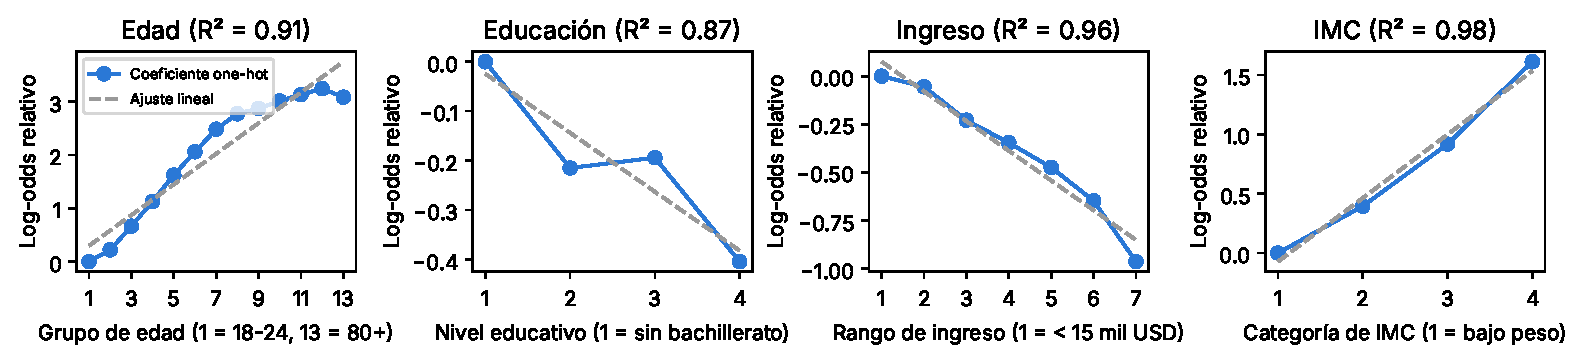
\includegraphics[width=0.94\textwidth]{proporcionalidad_ordinales.pdf}
\caption{Coeficientes de la regresión logística con codificación \textit{one-hot} para cada categoría de las variables ordinales, relativos a la primera categoría (línea continua), y su ajuste lineal (línea discontinua). Un ajuste lineal perfecto indicaría que tratar la variable como entero no pierde información.}
\label{fig:prop}
\end{figure*}

\subsubsection{Metodología de validación}
Los 342.539 registros se dividieron de forma estratificada en entrenamiento (80\%, 274.031) y prueba (20\%, 68.508); la prueba se apartó desde el inicio y se usó una sola vez. Atendiendo al costo computacional, la búsqueda de hiperparámetros se hizo con validación cruzada estratificada de 5 pliegues sobre una submuestra estratificada de 20.000 registros de entrenamiento, que conserva el 15,13\% de positivos: la SVM con kernel RBF escala de forma cuadrática con el número de muestras y tardó más de 15 minutos solo en esa malla. Cada métrica se reporta como la media de los 5 pliegues con su intervalo de confianza (IC) del 95\%, $\bar{x} \pm t_{0{,}975;\,4}\, s/\sqrt{5}$. Con los mejores hiperparámetros, cada modelo se reajustó con todo el entrenamiento y se evaluó en prueba, salvo la SVM, que se reajustó con una submuestra estratificada de 40.000 registros. En prueba, los IC se estimaron con 1.000 remuestreos \textit{bootstrap}.

\subsubsection{Manejo del desbalance}
Toda corrección del desbalance va dentro del \textit{pipeline}, así que se aplica solo a los pliegues de entrenamiento; validación y prueba conservan la proporción real de clases. La regresión logística, el bosque aleatorio y la SVM usan ponderación de clases inversamente proporcional a su frecuencia. KNN y el perceptrón multicapa no admiten ponderación en \textit{scikit-learn} y usan submuestreo aleatorio de la clase mayoritaria. El Cuadro~\ref{tab:balanceo} sustenta esta elección.

\subsubsection{Modelos e hiperparámetros}
Se compararon cinco modelos, uno por familia: regresión logística con regularización L2 (paramétrico), $k$ vecinos más cercanos (no paramétrico), bosque aleatorio (ensamble de árboles), perceptrón multicapa (red neuronal; ReLU, Adam y parada temprana) y SVM con kernel RBF. El Cuadro~\ref{tab:malla} presenta las mallas: 69 combinaciones, cada una evaluada en los 5 pliegues.

\begin{table}[!t]
\centering
\caption{Malla de hiperparámetros de cada modelo y valor elegido por mayor AUC de validación}
\label{tab:malla}
\footnotesize
\setlength{\tabcolsep}{3pt}
\begin{tabular}{@{}p{1.75cm}p{1.9cm}p{3.25cm}p{1.1cm}@{}}
\toprule
\textbf{Modelo} & \textbf{Parámetro} & \textbf{Valores} & \textbf{Elegido} \\
\midrule
Reg. logística & $C$ & $10^{-3}, 10^{-2}, \ldots, 10^{2}$ & 1 \\
\addlinespace
KNN & Vecinos $k$ & 5, 15, 31, 51, 101, 201, 401 & 401 \\
 & Pesos & uniforme, distancia & uniforme \\
\addlinespace
Bosque & N.º de árboles & 100, 300 & 100 \\
aleatorio & Prof. máxima & 4, 8, 12, sin límite & 12 \\
 & Mín. por hoja & 1, 10, 50 & 10 \\
\addlinespace
Red neuronal & Capas ocultas & (16), (64), (32, 16), (64, 32) & (16) \\
(MLP) & $\alpha$ (L2) & $10^{-4}, 10^{-2}, 10^{-1}, 1$ & $10^{-4}$ \\
\addlinespace
SVM (RBF) & $C$ & 0,1; 1; 10 & 1 \\
 & $\gamma$ & $10^{-3}, 10^{-2}, 10^{-1}$ & $10^{-2}$ \\
\bottomrule
\end{tabular}
\end{table}

\subsubsection{Métricas de desempeño}
Los hiperparámetros se eligen por el área bajo la curva ROC (AUC), que no depende del umbral de decisión ni de la proporción de clases. La sensibilidad es la métrica de monitoreo clave: en tamizaje, un falso negativo es una persona con diabetes que no se remite a evaluación, mientras que un falso positivo solo implica un examen adicional. Se reportan además la especificidad, que mide el costo en falsas alarmas, la precisión y el F1. La exactitud no se usa como criterio, porque un modelo que siempre predice ``no'' llegaría a 84,87\% sin detectar un solo caso.

\subsection{Resultados del entrenamiento de modelos}

\subsubsection{Codificación y desbalance}
Según el Cuadro~\ref{tab:codificacion}, la mejor codificación depende del modelo. La regresión logística pierde AUC al tratar las ordinales como enteros (0,66 puntos porcentuales, pp, con B; $p<0{,}01$), lo que coincide con la falta de proporcionalidad de la edad (Fig.~\ref{fig:prop}). Los modelos basados en distancias, en cambio, mejoran: KNN gana 4,24 pp con B ($p<0{,}01$) y la SVM 1,44 pp con C ($p<0{,}01$), porque así dos grupos de edad contiguos quedan más cerca que dos lejanos, mientras que en \textit{one-hot} todas las categorías están a la misma distancia. En el bosque aleatorio y la red neuronal las diferencias no son significativas y se conserva A.

\begin{table}[!t]
\centering
\caption{AUC de validación (media $\pm$ IC 95\%) según la codificación, y mayor diferencia frente a A en puntos porcentuales (pp). En negrita, la codificación adoptada}
\label{tab:codificacion}
\footnotesize
\setlength{\tabcolsep}{3pt}
\begin{tabular}{@{}lcccc@{}}
\toprule
\textbf{Modelo} & \textbf{A} & \textbf{B} & \textbf{C} & \textbf{Dif. (valor $p$)} \\
\midrule
Reg. logística & \textbf{0,76\,$\pm$\,0,01} & 0,75\,$\pm$\,0,01 & 0,75\,$\pm$\,0,01 & B: $-$0,66 (\textless 0,01) \\
KNN & 0,70\,$\pm$\,0,01 & \textbf{0,74\,$\pm$\,0,01} & 0,73\,$\pm$\,0,01 & B: +4,24 (\textless 0,01) \\
Bosque aleatorio & \textbf{0,75\,$\pm$\,0,01} & 0,75\,$\pm$\,0,01 & 0,75\,$\pm$\,0,01 & C: +0,35 (0,13) \\
Red neuronal & \textbf{0,75\,$\pm$\,0,01} & 0,75\,$\pm$\,0,01 & 0,75\,$\pm$\,0,02 & B: +0,06 (0,80) \\
SVM (RBF) & 0,73\,$\pm$\,0,01 & 0,75\,$\pm$\,0,01 & \textbf{0,75\,$\pm$\,0,01} & C: +1,44 (\textless 0,01) \\
\bottomrule
\end{tabular}
\end{table}

Sin corrección del desbalance (Cuadro~\ref{tab:balanceo}) los modelos conservan el AUC, pero casi no detectan positivos: la sensibilidad de la regresión logística cae a 0,04 y la del bosque a 0,00. SMOTE no mejora frente a la ponderación de clases: en la regresión logística baja el AUC 0,38 pp ($p<0{,}01$) y la sensibilidad 1,02 pp ($p=0{,}03$), y en el bosque la sensibilidad cae 29,87 pp ($p<0{,}01$). SMOTEN, la variante para variables categóricas, es la peor opción, con pérdidas de AUC cercanas a 4 pp. El submuestreo aleatorio rinde como la ponderación, lo que respalda su uso en KNN y la red neuronal.

\begin{table}[!t]
\centering
\caption{Desempeño en validación (media $\pm$ IC 95\%) según la estrategia para el desbalance de clases}
\label{tab:balanceo}
\footnotesize
\setlength{\tabcolsep}{3pt}
\begin{tabular}{@{}lccc@{}}
\toprule
\textbf{Estrategia} & \textbf{AUC} & \textbf{Sensibilidad} & \textbf{Especificidad} \\
\midrule
\multicolumn{4}{@{}l}{\textit{Regresión logística}} \\
\quad Sin corrección & 0,76\,$\pm$\,0,01 & 0,04\,$\pm$\,0,01 & 0,99\,$\pm$\,0,00 \\
\quad Ponderación de clases & 0,76\,$\pm$\,0,01 & 0,75\,$\pm$\,0,01 & 0,64\,$\pm$\,0,01 \\
\quad SMOTE & 0,75\,$\pm$\,0,01 & 0,74\,$\pm$\,0,02 & 0,64\,$\pm$\,0,01 \\
\quad SMOTEN & 0,72\,$\pm$\,0,01 & 0,64\,$\pm$\,0,02 & 0,67\,$\pm$\,0,00 \\
\quad Submuestreo aleatorio & 0,76\,$\pm$\,0,01 & 0,74\,$\pm$\,0,01 & 0,64\,$\pm$\,0,02 \\
\multicolumn{4}{@{}l}{\textit{Bosque aleatorio}} \\
\quad Sin corrección & 0,74\,$\pm$\,0,01 & 0,00\,$\pm$\,0,00 & 1,00\,$\pm$\,0,00 \\
\quad Ponderación de clases & 0,75\,$\pm$\,0,01 & 0,72\,$\pm$\,0,02 & 0,65\,$\pm$\,0,02 \\
\quad SMOTE & 0,74\,$\pm$\,0,01 & 0,42\,$\pm$\,0,03 & 0,84\,$\pm$\,0,01 \\
\quad SMOTEN & 0,71\,$\pm$\,0,01 & 0,53\,$\pm$\,0,02 & 0,75\,$\pm$\,0,01 \\
\quad Submuestreo aleatorio & 0,74\,$\pm$\,0,01 & 0,72\,$\pm$\,0,01 & 0,63\,$\pm$\,0,02 \\
\bottomrule
\end{tabular}
\end{table}

\subsubsection{Efecto de los hiperparámetros}
La Fig.~\ref{fig:hiper} muestra el AUC de entrenamiento y validación a lo largo de cada malla. En la regresión logística (a) solo la regularización más fuerte ($C=10^{-3}$) produce subajuste; desde $C=0{,}1$ el modelo ya no cambia. En KNN (b) el AUC de validación crece con $k$ hasta estabilizarse alrededor de $k=200$, y la ponderación por distancia sobreajusta: con datos categóricos abundan los vecinos a distancia cero, que reciben peso infinito. El bosque aleatorio (c) memoriza los datos cuando los árboles crecen sin límite y con hojas de una muestra, y se corrige al limitar la profundidad o exigir al menos 10 muestras por hoja; pasar de 100 a 300 árboles no cambia nada. La red neuronal (d) es poco sensible a la arquitectura y a $\alpha$, pues todas las combinaciones quedan dentro del IC de las demás. En la SVM (e), $\gamma=0{,}1$ con $C=10$ sobreajusta (AUC de 0,88 en entrenamiento y 0,71 en validación), mientras que $\gamma \leq 10^{-2}$ da fronteras suaves que generalizan mejor.

\begin{figure*}[!t]
\centering
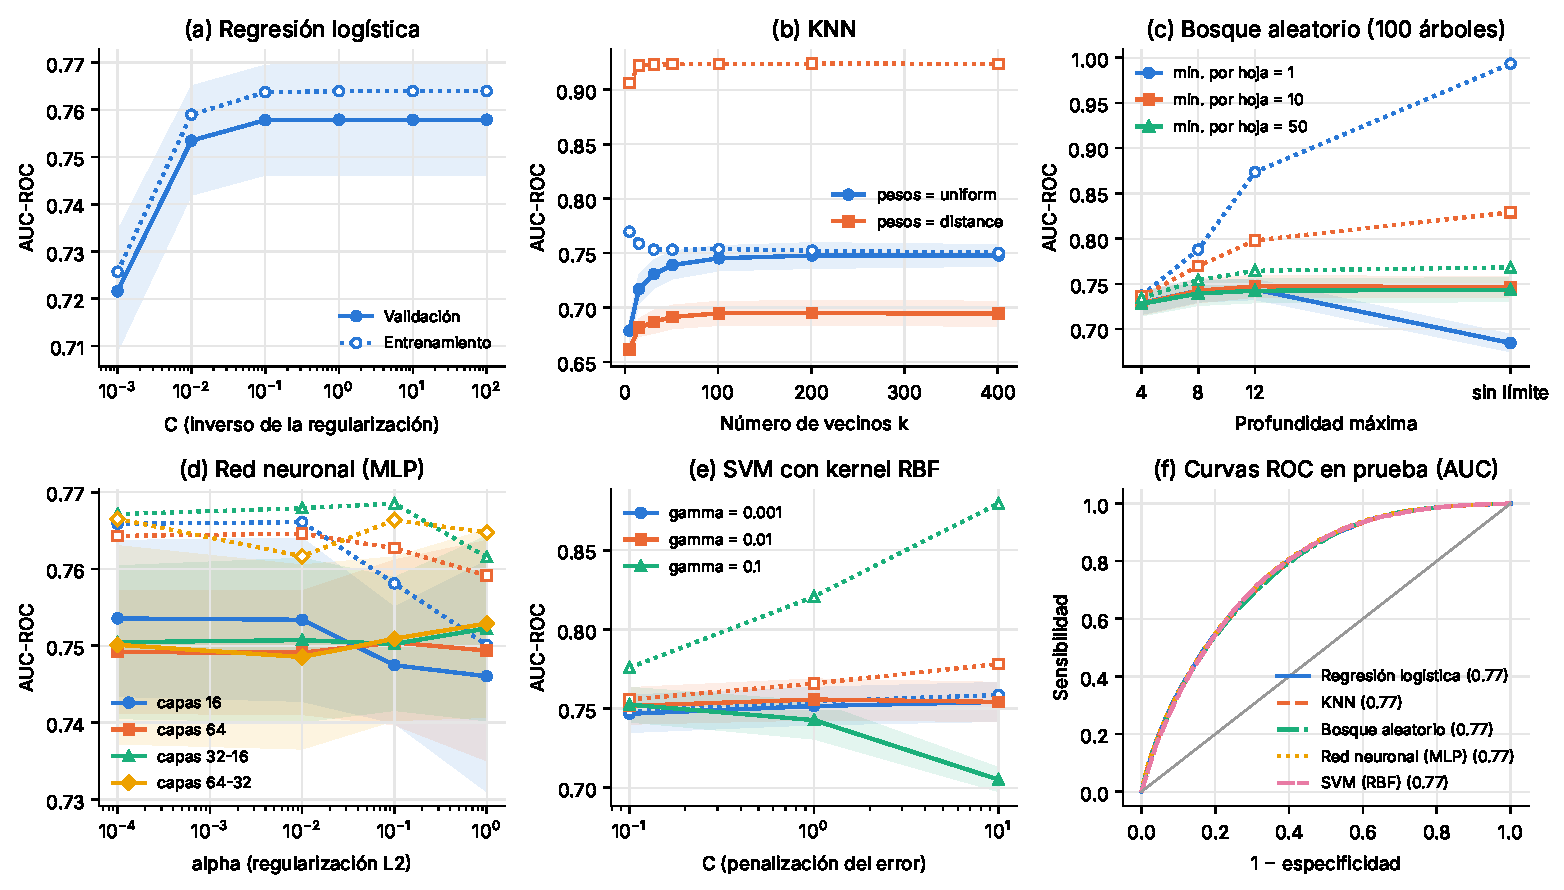
\includegraphics[width=0.9\textwidth]{hiperparametros_y_roc.pdf}
\caption{Efecto de los hiperparámetros sobre el AUC-ROC en la validación cruzada de 5 pliegues: (a) regresión logística, (b) KNN, (c) bosque aleatorio, (d) red neuronal y (e) SVM. La línea continua es la media de validación y la banda su IC del 95\%; la línea punteada es la media de entrenamiento. (f) Curvas ROC de los cinco modelos finales en el conjunto de prueba, con su AUC entre paréntesis.}
\label{fig:hiper}
\end{figure*}

\subsubsection{Desempeño final}
El Cuadro~\ref{tab:resultados} resume cada modelo con sus mejores hiperparámetros. En validación el AUC va de 0,75 a 0,76, con intervalos que se traslapan, y en prueba los cinco llegan a 0,77: ninguna familia es superior a las demás, y las curvas ROC son prácticamente indistinguibles (Fig.~\ref{fig:hiper}f). Esto sugiere que el techo lo ponen las once variables de encuesta y no la complejidad del modelo. El valor queda dentro del rango de 0,72 a 0,79 que reportan Xie et al. \cite{xie2019} con la misma encuesta. El AUC de prueba es algo mayor que el de validación porque los modelos finales se ajustan con muchos más datos (274.031 registros frente a 16.000 por pliegue). Solo el bosque aleatorio muestra una brecha apreciable entre entrenamiento y validación (0,80 frente a 0,75), que no se traduce en un peor resultado en prueba.

\begin{table*}[!t]
\centering
\caption{Desempeño de los cinco modelos con sus mejores hiperparámetros. Entrenamiento (Ent.) y validación (Val.): media $\pm$ IC 95\% sobre los 5 pliegues. Prueba: evaluación única; el AUC y la sensibilidad incluyen su IC 95\% por \textit{bootstrap}}
\label{tab:resultados}
\footnotesize
\setlength{\tabcolsep}{3.3pt}
\begin{tabular}{@{}lcccccccccc@{}}
\toprule
 & \multicolumn{3}{c}{\textbf{AUC-ROC}} & \multicolumn{3}{c}{\textbf{Sensibilidad}} & \multicolumn{2}{c}{\textbf{Especificidad}} & \multicolumn{2}{c}{\textbf{F1}} \\
\cmidrule(lr){2-4} \cmidrule(lr){5-7} \cmidrule(lr){8-9} \cmidrule(l){10-11}
\textbf{Modelo} & Ent. & Val. & Prueba & Ent. & Val. & Prueba & Val. & Prueba & Val. & Prueba \\
\midrule
Regresión logística & 0,76\,$\pm$\,0,00 & 0,76\,$\pm$\,0,01 & 0,77 [0,76; 0,77] & 0,76\,$\pm$\,0,01 & 0,75\,$\pm$\,0,01 & 0,75 [0,74; 0,76] & 0,64\,$\pm$\,0,01 & 0,65 & 0,40\,$\pm$\,0,01 & 0,40 \\
KNN & 0,75\,$\pm$\,0,00 & 0,75\,$\pm$\,0,01 & 0,77 [0,76; 0,77] & 0,74\,$\pm$\,0,01 & 0,74\,$\pm$\,0,01 & 0,77 [0,76; 0,78] & 0,63\,$\pm$\,0,02 & 0,63 & 0,39\,$\pm$\,0,01 & 0,40 \\
Bosque aleatorio & 0,80\,$\pm$\,0,00 & 0,75\,$\pm$\,0,01 & 0,77 [0,76; 0,77] & 0,78\,$\pm$\,0,01 & 0,72\,$\pm$\,0,02 & 0,74 [0,73; 0,75] & 0,65\,$\pm$\,0,01 & 0,65 & 0,39\,$\pm$\,0,01 & 0,40 \\
Red neuronal (MLP) & 0,77\,$\pm$\,0,00 & 0,75\,$\pm$\,0,01 & 0,77 [0,77; 0,78] & 0,76\,$\pm$\,0,02 & 0,74\,$\pm$\,0,03 & 0,77 [0,76; 0,78] & 0,64\,$\pm$\,0,02 & 0,64 & 0,39\,$\pm$\,0,01 & 0,40 \\
SVM (RBF) & 0,77\,$\pm$\,0,00 & 0,76\,$\pm$\,0,01 & 0,77 [0,76; 0,77] & 0,79\,$\pm$\,0,00 & 0,78\,$\pm$\,0,01 & 0,80 [0,80; 0,81] & 0,61\,$\pm$\,0,01 & 0,60 & 0,39\,$\pm$\,0,01 & 0,40 \\
\bottomrule
\end{tabular}
\end{table*}

En la métrica clave hay más diferencia. La Fig.~\ref{fig:confusion} presenta las matrices de confusión en prueba normalizadas por la clase real, de modo que la diagonal es directamente la sensibilidad y la especificidad. La SVM detecta el 80\% de las personas con diabetes, contra 74\% a 77\% de los demás modelos, a cambio de la especificidad más baja (0,60). Todos superan con amplitud el 51,6\% que obtuvieron Xie et al. \cite{xie2019}. El costo común es una precisión de 0,26 a 0,28: cerca de una de cada cuatro alertas corresponde a un caso real, algo esperable con 15\% de prevalencia y aceptable para un tamizaje cuyo siguiente paso es un examen de bajo costo.

\begin{figure*}[!t]
\centering
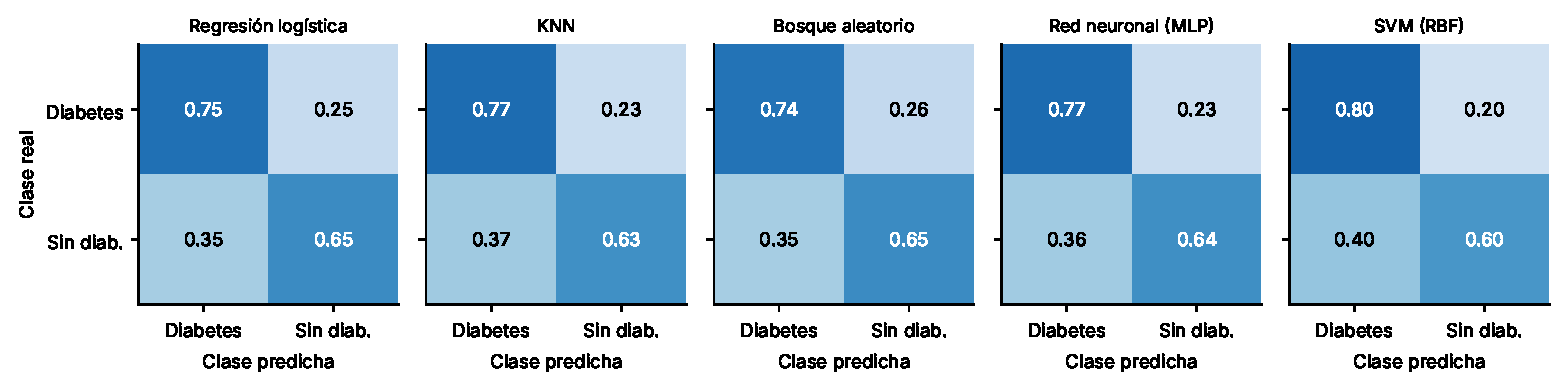
\includegraphics[width=0.92\textwidth]{matrices_confusion_normalizadas.pdf}
\caption{Matrices de confusión en el conjunto de prueba (68.508 registros), normalizadas por fila: cada celda es la fracción de la clase real que el modelo asigna a cada clase predicha.}
\label{fig:confusion}
\end{figure*}

Por último, se evaluó \texttt{LinearSVC}, que escala casi linealmente con el número de muestras. Con la codificación C su AUC de validación es 0,75\,$\pm$\,0,01 para cualquier $C$ entre 0,01 y 1, y ajustado con los 274.031 registros de entrenamiento en 1,3~s llega en prueba a un AUC de 0,76, sensibilidad de 0,73 y especificidad de 0,66. La SVM RBF, ajustada con 40.000 registros, tarda unos 5 minutos pero alcanza 0,77 de AUC y 7 puntos más de sensibilidad. Como la sensibilidad es la prioridad, se conservó el kernel RBF y se controló su costo con submuestras.

Los dos modelos con mayor AUC medio de validación, la regresión logística y la SVM (ambos 0,76), pasan a la fase de reducción de dimensión. La red neuronal queda muy cerca y la diferencia no es significativa, pero la SVM tiene además la mejor sensibilidad, y las dos elegidas representan enfoques distintos: una frontera lineal sobre variables \textit{one-hot} y una frontera no lineal sobre variables ordinales.


\section{Reducción de Dimensión}\label{sec:reduccion}
Todo el análisis de esta sección se hizo con el conjunto de entrenamiento, y las evaluaciones usan los mismos 5 pliegues de la sección anterior, de modo que cada resultado se puede comparar con el modelo sin reducción mediante una prueba $t$ pareada.

\subsection{Análisis individual de variables}
Para medir la capacidad discriminativa de cada predictora por separado se usaron tres índices, con ``no reportado'' como una categoría más: la V de Cramér derivada de la prueba $\chi^2$ de independencia con la diabetes, que va de 0 a 1; la información mutua, y un AUC univariado, en el que cada categoría se reemplaza por la prevalencia de diabetes observada en ella (estimada fuera de pliegue). Con 274.031 registros las once pruebas $\chi^2$ resultan significativas ($p<0{,}01$), así que la decisión se basa en la magnitud de la asociación y no en el valor $p$.

\begin{figure*}[!t]
\centering
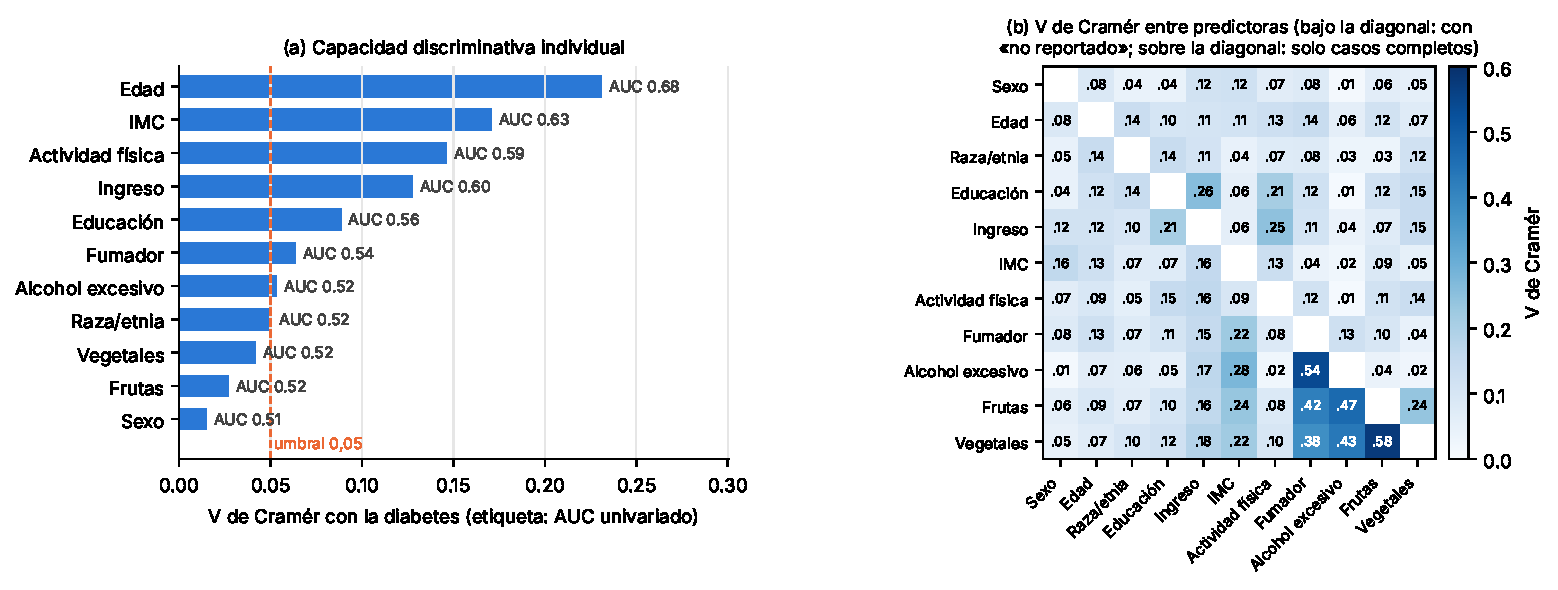
\includegraphics[width=0.9\textwidth]{analisis_individual.pdf}
\caption{(a) V de Cramér de cada predictora con la diabetes (barras) y su AUC univariado (etiqueta); la línea discontinua marca el umbral de 0,05 usado para señalar candidatas a eliminar. (b) V de Cramér entre pares de predictoras, calculada con ``no reportado'' como categoría (bajo la diagonal) y solo con los casos completos de cada par (sobre la diagonal).}
\label{fig:individual}
\end{figure*}

La Fig.~\ref{fig:individual}a ordena las variables. La edad es la más discriminativa por amplio margen (V = 0,23; AUC univariado de 0,68), seguida del IMC, la actividad física y el ingreso, lo que coincide con las variables de mayor peso que encontraron Majcherek et al. \cite{majcherek2025} con SHAP. En el otro extremo, vegetales, frutas y sexo tienen V por debajo de 0,05 y AUC univariados de 0,51 a 0,52, prácticamente el de una clasificación al azar. Con el criterio V $<0{,}05$ y AUC univariado $<0{,}55$, esas tres son las candidatas a eliminar; raza/etnia y alcohol quedan justo por encima del umbral.

La redundancia entre predictoras (Fig.~\ref{fig:individual}b) parece alta en algunos pares cuando se incluye ``no reportado'': frutas y vegetales tienen V = 0,58 y fumador y alcohol, 0,54. Sin embargo, con los casos completos esos valores bajan a 0,24 y 0,13. La asociación se debe sobre todo a que las mismas personas dejan sin responder varias preguntas de estilo de vida, no a que los hábitos se repitan entre sí. Ningún par supera 0,5 con casos completos, así que no se eliminó ninguna variable por redundancia.

Al retirar las tres candidatas, la regresión logística pasa de 57 a 49 columnas (14\% menos) y la SVM de 39 a 29 (26\% menos). El AUC de validación baja 0,12 pp en la regresión logística ($p=0{,}28$) y 0,20 pp en la SVM ($p=0{,}09$), diferencias que no son significativas, y la sensibilidad no cambia (Cuadro~\ref{tab:reduccion}). Vale la pena anotar que retirar solo el sexo de la SVM sí produce una caída pequeña pero significativa (0,25 pp; $p=0{,}04$): por sí solo casi no discrimina, pero el modelo no lineal parece aprovecharlo en combinación con otras variables, como el IMC.

\subsection{Extracción lineal de características: PCA}
PCA se insertó en el \textit{pipeline} justo después de la codificación, de modo que en cada pliegue los componentes se calculan solo con los datos de entrenamiento del pliegue. Para cada modelo se recorrió el número de componentes $k$ y se aplicó este criterio: el menor $k$ cuyo AUC de validación no sea significativamente menor que el del modelo sin reducción (prueba $t$ pareada, $p\geq0{,}05$) y cuya pérdida media no supere 0,5 pp. Se prefirió a un umbral fijo de varianza explicada porque en datos codificados la varianza no tiene por qué concentrarse en las direcciones que separan las clases, y aquí lo que importa es no perder capacidad de detección.

La Fig.~\ref{fig:pcaumap} muestra el resultado. En la regresión logística el AUC sube muy despacio con $k$: con 10 componentes, menos que las once variables originales, cae a 0,67, y el criterio solo se cumple con $k=45$ (AUC 0,76; $p=0{,}60$). Hay una razón estructural: las 57 columnas \textit{one-hot} suman 1 dentro de cada una de las once variables, así que su rango es 46, y 45 componentes equivalen casi al espacio completo. Además, la información de la edad, la variable más útil, está repartida en 14 columnas binarias de poca varianza cada una, y PCA, que solo atiende a la varianza, no tiene por qué conservarla en los primeros componentes. En la SVM, con edad, educación, ingreso e IMC como columnas estandarizadas, los primeros componentes sí recogen esa información: con 4 componentes el AUC ya es 0,74, y el criterio se cumple con $k=20$ (AUC 0,76; $p=0{,}35$; 98\% de la varianza), la mitad de las 39 columnas. Con $k=10$ la pérdida es de 1,09 pp y resulta significativa ($p<0{,}01$).

\begin{figure*}[!t]
\centering
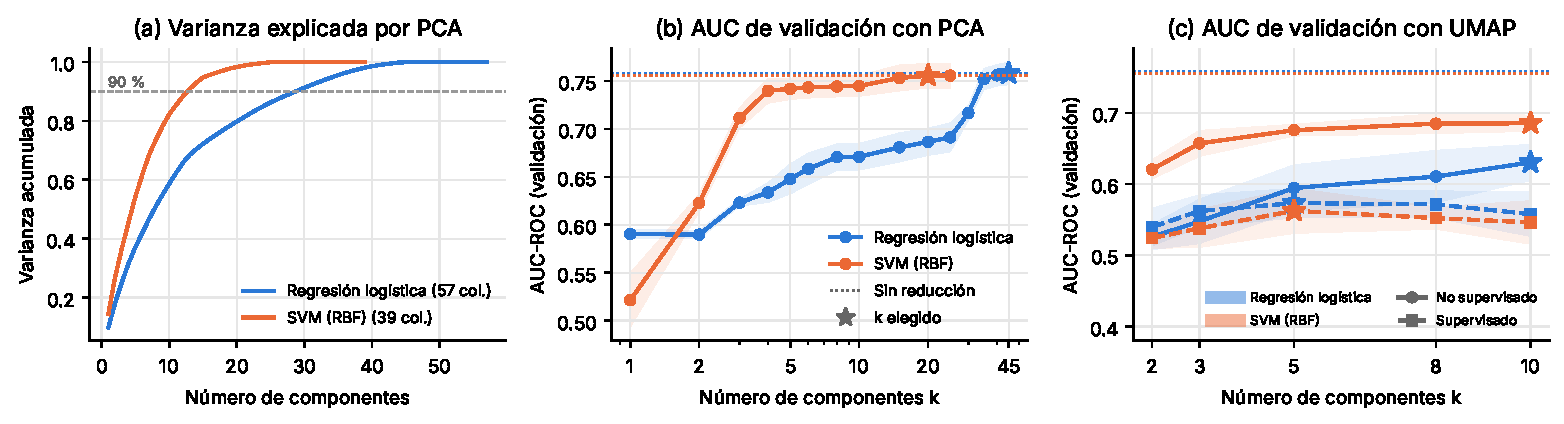
\includegraphics[width=0.92\textwidth]{pca_umap_componentes.pdf}
\caption{(a) Varianza explicada acumulada por PCA sobre la codificación de cada modelo. (b) y (c) AUC de validación (media e IC del 95\% en 5 pliegues) según el número de componentes con PCA y con UMAP; la línea punteada es el AUC sin reducción y la estrella marca el $k$ elegido con el criterio de no pérdida significativa.}
\label{fig:pcaumap}
\end{figure*}

\subsection{Extracción no lineal de características: UMAP}
UMAP construye un grafo de vecinos en el espacio codificado y busca una representación de baja dimensión que lo conserve. Se insertó en el mismo lugar del \textit{pipeline} que PCA, con \texttt{n\_neighbors} = 30, \texttt{min\_dist} = 0 (recomendado cuando el resultado se usa para clasificar y no para visualizar) y métrica euclidiana, y las coordenadas resultantes se estandarizaron antes del clasificador. Como la geometría cambia, se reajustó un hiperparámetro de cada modelo ($C\in\{0{,}01; 1\}$ en la regresión logística y $\gamma\in\{0{,}1;$ \texttt{scale}$\}$ en la SVM). Se recorrió $k\in\{2, 3, 5, 8, 10\}$, siempre por debajo de las once variables originales, con el mismo criterio de PCA. Además de la versión estándar, no supervisada, se probó UMAP supervisado, que al construir el grafo también usa la etiqueta, pero solo la de los registros de entrenamiento de cada pliegue; validación y prueba se proyectan sin etiqueta.

Ningún $k$ cumple el criterio (Fig.~\ref{fig:pcaumap}c). Con UMAP no supervisado el AUC de validación crece con $k$, pero con 10 componentes apenas llega a 0,63 en la regresión logística y 0,69 en la SVM, entre 7 y 13 pp por debajo del modelo sin reducción, así que se tomó $k=10$, el de mayor AUC. Una explicación probable es la naturaleza de los datos: once variables categóricas generan relativamente pocos perfiles distintos, con muchos registros idénticos, y el grafo de vecinos tiene que desempatar entre puntos a la misma distancia; además, UMAP conserva la estructura que domina el espacio codificado, que no tiene por qué ser la relacionada con la diabetes. La regresión logística sufre más porque el riesgo no es lineal en las coordenadas de UMAP, y el kernel RBF compensa una parte. La versión supervisada es peor todavía: el AUC de entrenamiento sube a 0,98, pero en validación no pasa de 0,57 y la sensibilidad cae por debajo de 0,20. El \textit{embedding} separa casi perfectamente a los registros de entrenamiento según su etiqueta, mientras que un registro nuevo, sin etiqueta, cae entre vecinos de ambas clases; es un sobreajuste del propio paso de reducción.

\begin{table*}[!t]
\centering
\caption{Desempeño de los dos mejores modelos con cada técnica de reducción. Dim.: número de columnas o componentes que recibe el clasificador; Red.: reducción frente a las columnas de la codificación original (57 en la regresión logística y 39 en la SVM). Entrenamiento y validación: media $\pm$ IC 95\% en 5 pliegues; prueba: valor con IC 95\% por \textit{bootstrap}}
\label{tab:reduccion}
\footnotesize
\setlength{\tabcolsep}{3.5pt}
\begin{tabular}{@{}lcccccccccc@{}}
\toprule
 & & & \multicolumn{3}{c}{\textbf{AUC-ROC}} & \multicolumn{2}{c}{\textbf{Sensibilidad}} & & \\
\cmidrule(lr){4-6} \cmidrule(lr){7-8}
\textbf{Versión} & \textbf{Dim.} & \textbf{Red.} & Ent. & Val. & Prueba & Val. & Prueba & \textbf{Espec.} & \textbf{F1} \\
\midrule
\multicolumn{10}{@{}l}{\textit{Regresión logística}} \\
\quad Sin reducción & 57 & -- & 0,76\,$\pm$\,0,00 & 0,76\,$\pm$\,0,01 & 0,77 [0,76; 0,77] & 0,75\,$\pm$\,0,01 & 0,75 [0,74; 0,76] & 0,65 & 0,40 \\
\quad Sin sexo, frutas y vegetales & 49 & 14\% & 0,76\,$\pm$\,0,00 & 0,76\,$\pm$\,0,01 & 0,77 [0,76; 0,77] & 0,75\,$\pm$\,0,02 & 0,74 [0,74; 0,75] & 0,65 & 0,40 \\
\quad PCA & 45 & 21\% & 0,76\,$\pm$\,0,00 & 0,76\,$\pm$\,0,01 & 0,77 [0,76; 0,77] & 0,75\,$\pm$\,0,01 & 0,75 [0,74; 0,76] & 0,65 & 0,40 \\
\quad PCA & 10 & 82\% & 0,67\,$\pm$\,0,00 & 0,67\,$\pm$\,0,01 & 0,68 [0,68; 0,69] & 0,60\,$\pm$\,0,02 & 0,62 [0,61; 0,63] & 0,65 & 0,34 \\
\quad UMAP & 10 & 82\% & 0,63\,$\pm$\,0,01 & 0,63\,$\pm$\,0,03 & 0,60 [0,60; 0,61] & 0,60\,$\pm$\,0,03 & 0,56 [0,55; 0,57] & 0,60 & 0,29 \\
\quad UMAP supervisado & 5 & 91\% & 0,98\,$\pm$\,0,00 & 0,57\,$\pm$\,0,02 & 0,62 [0,61; 0,62] & 0,10\,$\pm$\,0,02 & 0,18 [0,17; 0,18] & 0,92 & 0,22 \\
\multicolumn{10}{@{}l}{\textit{SVM (RBF)}} \\
\quad Sin reducción & 39 & -- & 0,77\,$\pm$\,0,00 & 0,76\,$\pm$\,0,01 & 0,77 [0,76; 0,77] & 0,78\,$\pm$\,0,01 & 0,80 [0,80; 0,81] & 0,60 & 0,40 \\
\quad Sin sexo, frutas y vegetales & 29 & 26\% & 0,76\,$\pm$\,0,00 & 0,75\,$\pm$\,0,01 & 0,76 [0,76; 0,77] & 0,78\,$\pm$\,0,01 & 0,80 [0,79; 0,81] & 0,60 & 0,39 \\
\quad PCA & 20 & 49\% & 0,76\,$\pm$\,0,00 & 0,76\,$\pm$\,0,01 & 0,77 [0,76; 0,77] & 0,78\,$\pm$\,0,01 & 0,80 [0,80; 0,81] & 0,60 & 0,40 \\
\quad PCA & 10 & 74\% & 0,75\,$\pm$\,0,00 & 0,74\,$\pm$\,0,01 & 0,76 [0,75; 0,76] & 0,77\,$\pm$\,0,01 & 0,81 [0,80; 0,82] & 0,57 & 0,38 \\
\quad UMAP & 10 & 74\% & 0,70\,$\pm$\,0,00 & 0,69\,$\pm$\,0,01 & 0,69 [0,69; 0,70] & 0,71\,$\pm$\,0,04 & 0,70 [0,69; 0,71] & 0,59 & 0,35 \\
\quad UMAP supervisado & 5 & 87\% & 0,98\,$\pm$\,0,00 & 0,56\,$\pm$\,0,03 & 0,55 [0,55; 0,56] & 0,08\,$\pm$\,0,01 & 0,14 [0,13; 0,14] & 0,95 & 0,19 \\
\bottomrule
\end{tabular}
\end{table*}

El Cuadro~\ref{tab:reduccion} reúne los resultados en prueba. Las tres versiones que no pierden desempeño en validación tampoco lo pierden en prueba: sin sexo, frutas y vegetales, con PCA de 45 componentes en la regresión logística y con PCA de 20 en la SVM, el AUC sigue en 0,76 a 0,77 y la sensibilidad en 0,74--0,75 y 0,80, respectivamente. Con 10 componentes, PCA le cuesta a la regresión logística 9 pp de AUC y 13 pp de sensibilidad, mientras que a la SVM solo 1 pp de AUC, con una sensibilidad similar (0,81) a cambio de 3 pp de especificidad. UMAP, en sus dos variantes, queda claramente por debajo, y la versión supervisada confirma en prueba el sobreajuste visto en validación (sensibilidad de 0,14 a 0,18).

\section{Discusión y Conclusiones}\label{sec:conclusiones}
Los cinco modelos terminan en el mismo lugar: AUC de 0,75 a 0,76 en validación y de 0,77 en prueba, con intervalos que se traslapan. Que una regresión logística iguale a una SVM con kernel o a una red neuronal indica que el límite lo pone la información disponible y no la capacidad del modelo. Once preguntas de encuesta, con el IMC agrupado en cuatro categorías, no alcanzan a describir el riesgo con más detalle. El resultado está dentro del rango de Xie et al. \cite{xie2019} con la misma encuesta; los AUC cercanos a 0,99 de otros trabajos \cite{majcherek2025} usan más variables, entre ellas la salud general percibida, y otra preparación de los datos, así que no son directamente comparables.

Donde sí hay diferencias es en la métrica clave. Con la ponderación de clases, todos los modelos detectan entre 74\% y 80\% de los casos en prueba, frente al 51,6\% de Xie et al.; la SVM es la que más detecta, a cambio de más falsas alarmas. SMOTE no mejoró frente a la ponderación de clases y SMOTEN empeoró los resultados, lo que confirma que, con un desbalance moderado como este, ponderar las clases basta. También quedó claro que la codificación importa más de lo que parece: tratar las ordinales como enteros ayuda a los modelos de distancia pero perjudica a la regresión logística, porque el efecto de la edad no es proporcional, y conservar ``no reportado'' como categoría tiene sentido porque no responder se asocia con la diabetes en seis de las diez variables con faltantes.

La reducción de dimensión deja una conclusión práctica y otra metodológica. La práctica es que sexo, frutas y vegetales se pueden retirar sin perder desempeño: un cuestionario de tamizaje con ocho preguntas en lugar de once es más corto de aplicar, y eso tiene más valor en este contexto que ahorrar columnas. La metodológica es que las técnicas de extracción rinden muy distinto según la codificación. PCA no reduce de verdad la regresión logística, porque sus 45 componentes son casi el rango completo de la codificación \textit{one-hot}; en la SVM, que recibe las ordinales como números, 20 componentes conservan todo el desempeño y 10 pierden solo un punto de AUC, aunque a costa de que las nuevas variables ya no se pueden interpretar. UMAP no funcionó con estos datos categóricos, y su versión supervisada mostró que un paso de reducción también puede sobreajustar si se le da la etiqueta, algo que solo se detecta porque se evaluó dentro de la validación cruzada.

Con todo esto, la regresión logística sin sexo, frutas y vegetales es la opción más recomendable para un tamizaje: tiene el mismo AUC que cualquier otro modelo (0,77), detecta tres de cada cuatro casos, se entrena en un segundo con todos los datos y sus coeficientes se pueden explicar. Si la prioridad es detectar más casos aunque aumenten las falsas alarmas, la SVM llega a una sensibilidad de 0,80.

Este trabajo tiene limitaciones que conviene tener presentes. El diagnóstico es autorreportado, así que entre los negativos hay personas con diabetes no diagnosticada; los datos son transversales, de modo que el modelo identifica perfiles asociados con tener diabetes y no predice quién la desarrollará; no se usaron los pesos muestrales de la encuesta, y faltan cuatro jurisdicciones. Como trabajo futuro quedan ajustar el umbral de decisión para fijar una sensibilidad objetivo, calibrar las probabilidades e incorporar variables como la salud general percibida, la hipertensión o el colesterol, que el BRFSS también recoge.



\begin{thebibliography}{4}

\bibitem{xie2019}
Z. Xie, O. Nikolayeva, J. Luo, and D. Li, ``Building risk prediction models for type 2 diabetes using machine learning techniques,'' \emph{Prev. Chronic Dis.}, vol. 16, Art. no. 190109, 2019, doi: 10.5888/pcd16.190109.

\bibitem{majcherek2025}
D. Majcherek, A. Ciesielski, and P. Sobczak, ``AI-driven analysis of diabetes risk determinants in U.S. adults: Exploring disease prevalence and health factors,'' \emph{PLoS ONE}, vol. 20, no. 9, Art. no. e0328655, Sep. 2025, doi: 10.1371/journal.pone.0328655.

\bibitem{chowdhury2024}
M. M. Chowdhury, R. S. Ayon, and M. S. Hossain, ``An investigation of machine learning algorithms and data augmentation techniques for diabetes diagnosis using class imbalanced BRFSS dataset,'' \emph{Healthcare Analytics}, vol. 5, Art. no. 100297, Jun. 2024, doi: 10.1016/j.health.2023.100297.

\bibitem{ekambaram2026}
G. Ekambaram, T. Rakkiannan, N. Palanisamy, S. Muthusamy, A. Singh, K. K. Sadasivuni, and M. Krishnamoorthy, ``A novel method for early detection and prediction of diabetes using various machine learning and deep learning models,'' \emph{Int. J. Diabetes Dev. Ctries.}, vol. 46, pp. 278--295, Mar. 2026, doi: 10.1007/s13410-025-01590-y.

\end{thebibliography}

\end{document}
